\documentclass[compress,mathserif,serif]{beamer}

%\usetheme{Berkeley}

\usepackage{dsfont,calc,xcolor,amsfonts,amsthm,amscd,epsfig,psfrag,amsmath,amssymb,mathtools,commath,enumerate,srcltx,graphicx,xmpmulti}
\usepackage{pgf,tikz}
\usepackage{mathrsfs}
\usetikzlibrary{arrows}
\usetikzlibrary{shapes,backgrounds,positioning,fit}
\usepackage[accumulated]{beamerseminar}
\usepackage{pdfpages}


\usepackage{beamerthemeshadow}


\usepackage{pgfpages}
%\setbeameroption{show notes on second screen=left}
%\setbeameroption{previous slide on second screen=left}


\newtheorem{thm}{Theorem}
\newtheorem{Cor}{Corollary}
\newtheorem{question}{Question}
\newtheorem{Con}{Lemma}
\newtheorem{dfn}{Definition}
\newtheorem{prop}{Proposition}
\newtheorem{remark}{Remark}
\newtheorem{Fact}{Fact}
\newtheorem{conn}{Conjecture}
\newtheorem{rem}{Remark}
\newtheorem{exm}{Example}
\usepackage[english]{babel}


\title{Geometry over Fields}
\author[Marco Bertenghi]{\bf Marco Bertenghi}
\institute[UZH]{\bf University of Zurich}


\newcommand{\sref}[1]{SLIDE \ref{#1}}
\setbeamertemplate{navigation symbols}{}
\setbeamertemplate{headline}{}


\usepackage{color}
\usepackage{graphicx}
\usepackage{amssymb}
\usepackage{amsmath}
\usepackage{latexsym}
\usepackage{amsthm}
\usepackage{mathrsfs}
\usepackage{colonequals}


\vspace{4 cm}
\date{}
\vspace{4 cm}

%%%%%%%%%%%%%%%%%%%%%%%%%%%%%%%%%%%%%%%%%%%%%%%%%%%%%
\begin{document}


\begin{frame}
\titlepage
\centerline{\textcolor{blue}{\bf 9th of April 2019}}
\vspace{0.5cm}
\end{frame}




\begin{frame}
\tableofcontents
\end{frame}

\section{Introduction}


\begin{frame}
\begin{center}
\Huge{\color{blue}{\bf{Introduction}}}
\end{center}
\end{frame}




\begin{frame}
\frametitle{Introduction}

\begin{itemize}
\item So far: 
\pause
\begin{itemize}
\item Purely axiomatic approach: i.e. geometrical postulates and proving results in a logical sequence from them.
\pause
\item The geometry developed in Euclid's \textit{Elements} does not make use of numbers to measure lengths or angles or areas.
\end{itemize}
\pause
\item Meanwhile:
\pause
\begin{itemize}
\item In the centuries after Euclid, geometers began using numbers more and more.
\pause
\item A big step was taken by Descartes (1596-1650), in his book
\textit{La Geometrie}:
construction of product, quotient, and square root of line
segments, having once fixed a unit line segment.
\pause
\begin{itemize}
\item $\rightsquigarrow$ Analytic geometry.
\end{itemize}
\end{itemize}
\end{itemize}
\end{frame}

\begin{frame}
\frametitle{Introduction}
\begin{itemize}
\item Still meanwhile:
\pause
\begin{itemize}
\item Concept of numbers were expanded:
\pause
\begin{itemize}
\item $\mathbb{N} \subset \mathbb{Z} \subset \mathbb{Q} \subset \mathbb{R}$.
\end{itemize}
\pause
\item End of 19th Century:
\pause
\begin{itemize}
\item Considerations of limit and continuity developed, which made $\mathbb{R}$ into the standard model for analytic geometry, calculus. 
\pause
\item Formalization of abstract structures in mathematics led to the concept of a field.
\pause
\item Standard model for field is still $\mathbb{R}$, but one could also consider a geometry over any abstract field.
\end{itemize}
\end{itemize}
\end{itemize}
\end{frame}

\begin{frame}
\frametitle{Introduction}
\begin{itemize}
\item Now: 
\pause
\begin{itemize}
\item Forget about Euclid.
\pause
\item Forget about Hilbert.
\pause
\item  Accept the field of real numbers $\mathbb{R}$ as given.
\pause 
\item Diverge from purely axiomatic track.
\pause
\begin{itemize}
\item Rather follow the algebraic methods of Descartes, that is the geometry over a field.
\pause
\item  In this framework the theory is built on a logical platform given by the algebraic definition of a field and its operations.
\end{itemize}
\end{itemize}
\end{itemize}
\end{frame}


\begin{frame}
\frametitle{Introduction}
\begin{itemize}
\item Goal for today:
\pause
\begin{itemize}
\item Introduce and study the real Cartesian plane.
\pause
\begin{itemize}
\item See some easy applications in this framework.
\pause
\item Descartes' theorem: \textit{richness} of the Cartesian plane.
\pause
\item Compare to earlier results and methods.
\end{itemize}
\pause
\item Study geometries over a general field.
\pause
\begin{itemize}
\item Tip: Finite Geometries I/II (ETHZ, 4+4 ECTS)
\end{itemize}
\pause
\item Possibly let the two frameworks (axiomatic and analytic) \textit{converge}. 
\end{itemize}
\end{itemize}
\end{frame}


\begin{frame}
\frametitle{Introduction}
Familiarity with:
\pause
\begin{itemize}
\item Quantum symplectic geometry.
\pause
\item Poisson geometry.
\pause
\item Voronoi Tessellation and its associated Percolation Model.
\end{itemize}
\pause
... are \textbf{absolutely not needed} to follow this talk. 
\pause
\begin{itemize}
\item Instead know some highschool (gymi) geometry.
\end{itemize}
\pause \textit{(Out of season April fools joke)}
\end{frame}

\section{The Real Cartesian Plane}

\begin{frame}
\begin{center}
\Huge{\color{blue}{\bf{The Real Cartesian Plane}}}
\end{center}
\end{frame}

\begin{frame}
\frametitle{The Real Cartesian Plane}
\begin{dfn}
We call a \textbf{point} an ordered pair $P=(a,b)$ of real numbers, and the set of all such ordered pairs is the Cartesian plane. We call the set of points $(a,0)$ the $x$-axis, and the set of points $(0,b)$ the $y$-axis. The intersection of the two axis $(0,0)$ is called the \textbf{origin}.
\end{dfn}
\pause
\begin{figure}[hbtp]
\centering
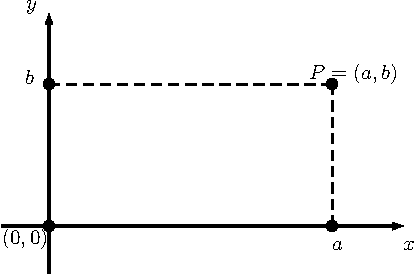
\includegraphics[scale=.9]{cartplane.pdf}
\end{figure}
\end{frame}

\begin{frame}
\frametitle{The Real Cartesian Plane}
\begin{dfn}A \textbf{line} in the Cartesian plane is the subset (of the Cartesian plane) defined by a linear equation of the form $ax+by+c=0$, with $a,b$ not both zero. We will write these lines in the canonical form $y=mx+q$, we call $m$ the \textbf{slope} of the line and $q$ its $y$-intercept. We call $x=a$ a vertical line and agree that it has slope $\infty$. 
\end{dfn}
\end{frame}


\begin{frame}
\frametitle{The Real Cartesian Plane}
\begin{dfn}Two lines $l_1,l_2$ are called \textbf{parallel}, denoted by $l_1 \| l_2$, if they are equal or if they have no points in common, i.e. $l_1 \cap l_2 = \emptyset$.
\end{dfn}
\pause
\begin{Con} Two lines are parallel if and only if they have the same slope.
\end{Con}
\pause
\begin{proof}
$\bullet$ If the lines are equal, then they have the same slope.
\pause
\newline
$\bullet$ If the lines are distinct, parallel, then the slope must be equal for else they would meet at a unique intersection point.
\pause
\newline $\bullet$ Converse arguments are the same. 
\pause
\newline $\bullet$ All of the above can be verified by looking at the equations for lines. 
\end{proof}
\end{frame}


\begin{frame}
\frametitle{The Real Cartesian Plane}
\begin{Cor}If $l_1,l_2,l_3$ are three distinct lines, and $l_1 \| l_2$ and $l_2 \| l_3$, then $l_1 \| l_3$.
\end{Cor}
\pause
\begin{proof}
Indeed, all three must have the same slope as a consequence of the previous Lemma.
\end{proof}
\pause
\begin{rem}
In Euclid's \textit{Elements}, this result appears as (I.30) and is proved there using the parallel postulate plus earlier results from Book I, in particular it is non-trivial. Here, in the Cartesian plane, we have a trivial proof just by looking at the equations of the lines.
\end{rem}
\end{frame}

\begin{frame}
\frametitle{The Real Cartesian Plane}
\begin{prop} In the real Cartesian plane, the three altitudes of any triangle all meet at a single point.
\end{prop}
\begin{figure}[hbtp]
\centering
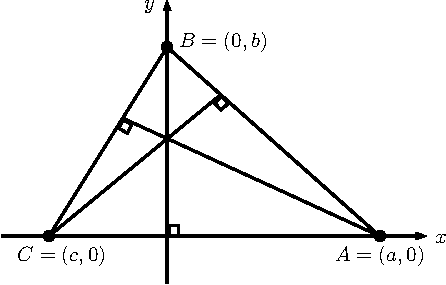
\includegraphics[scale=1]{prop1.pdf}
\end{figure}
\end{frame}



\begin{frame}
\frametitle{The Real Cartesian Plane}
\begin{proof}[Proof of Proposition]
\begin{figure}[hbtp]
\centering
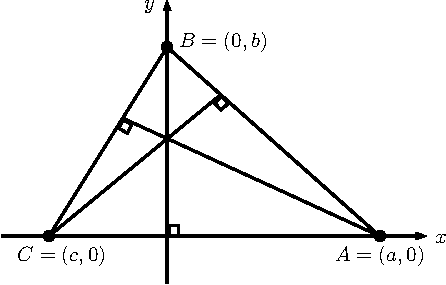
\includegraphics[scale=.7]{prop1.pdf}
\end{figure}
$\bullet$ W.l.o.g. we can arrange the triangle as depicted above. In particular the $y$-Axis will be one of the altitudes.
\pause
\newline $\bullet$ Idea: Find equations of two remaining altitudes and verify they meet the $y$-axis at same point.
\pause
\newline $\bullet$ To this end, use that two lines with perpendicular slope satisfy $m_1m_2=-1$.

\end{proof}

\end{frame}


\begin{frame}
\frametitle{The Real Cartesian Plane}
Let us reflect for a moment on the significance of this proof. If we compare this
particular proof with the one presented in Section 5 (Some Newer Results), we notice that there is quite a
difference in its
\textit{complexity}.
\pause 
\begin{question}How do we
respond to someone who says, with a simple analytic proof like the one presented before, why bother with geometric proofs from axioms?
\end{question}
\end{frame}

\begin{frame}
\frametitle{The Real Cartesian Plane}
\begin{question}How do we
respond to someone who says, with a simple analytic proof like the one presented before, why bother with geometric proofs from axioms?
\end{question}
\pause
Answer might be subtle:
\pause
\begin{itemize}
\item Modern maths has abandoned the naive position
that any framework is universally more potent than another
point of view. 
\pause
\begin{itemize}
\item Want to know what can be proved within each logical framework, within each separate mathematical theory. 
\end{itemize}
\pause
\item Since result holds in this framework, we expect it
to be true in the framework of axiomatic Euclidean geometry. But proof gives no insight about how to find a proof in the abstract axiomatic
geometry, or if proof even exists.
\end{itemize}
\end{frame}



\begin{frame}
\frametitle{The Real Cartesian Plane}
\begin{thm}[Descartes] Suppose we are given points $P_1=(a_1,b_1), \dots ,  P_n=(a_n,b_n)$ in the real Cartesian plane and also assume that we are given the points $(0,0)$ and $(1,0)$ (in order to construct a unit). Then it is possible to construct a point $Q= ( \alpha,  \beta)$ with ruler and compass if and only if $\alpha$ and $\beta$ can be obtained from $a_1, \dots , a_n, b_1, \dots , b_n$ by field operations $+,-, \cdot, \div$ and the solution of a finite number of successive linear and quadratic equations, involving the square roots of positive real numbers. 
\end{thm}
\pause
\begin{rem} Descartes discovered that the ruler and compass constructions of Euclid's geometry correspond to the solution of linear and quadratic equations in algebra.
\end{rem}
\end{frame}


\begin{frame}
\frametitle{The Real Cartesian Plane}
As Descartes said after the discovery of his theorem:
\newline
\newline
\textit{One can construct all the problems of ordinary geometry without doing anything more than what little is contained in the four figures which I am about to explain; which is something I do not believe that ancients had noticed: for otherwise they would not have taken the trouble to write so many fat books,  where already the order of their propositions makes it clear that they did not have the true method for finding them all,  but merely collected those which they happened to come across.}
\end{frame}


\begin{frame}
\frametitle{The Real Cartesian Plane}
\begin{proof}[Proof of Theorem]\let\qed\relax A ruler and compass construction consists of drawing
lines through given points, constructing circles with given center and radius,
and finding intersections of lines and circles.
\pause
\newline
\newline
$\bullet$ Given two points $P_1=(a_1,b_1)$ and $P_2=(a_2,b_2)$, the line passing through them has equation $ y-b_1= \frac{b_2-b_1}{a_2-a_1}(x-a_1).$ Its coefficients are obtained by field operations from the initial data $a_1,a_2,b_1,b_2$.
\pause
\newline
\newline
$\bullet$ A circle with center $(a,b)$ and radius $r$ has equation
  $(x-a)^2 + (y-b)^2=r^2.$
This is a quadratic equation whose coefficients depend on $a,b$ and $r$.
\end{proof}
\end{frame}


\begin{frame}
\frametitle{The Real Cartesian Plane}
\begin{proof}[Proof of Theorem]\let\qed\relax
$\bullet$ To find the intersection of two lines, we solve two linear equations, which can be done using only field operations.
\pause
\newline
\newline
$\bullet$ To intersect a line with a circle, we solve the equations simultaneously, which requires solving a quadratic eqn. in $x$.
\pause
\newline
\newline
$\bullet$ To intersect two circles, we first subtract the two equations, which eliminates the $x^2$ and $y^2$ terms. Then we must solve a quadratic equation with a linear equation, leading to another quadratic equation in $x$.
\pause
\newline
\newline
$\bullet$ Summary: to find the coordinates point $Q=( \alpha, \beta)$ obtained by a ruler and compass from the initial data $P_1, \dots , P_n$, we must solve a finite number of linear and quadratic eqn. whose coefficients depend on the coordinates $(a_i,b_i)$ and on quantities constructed the steps above.
\end{proof}
\end{frame}


\begin{frame}
\frametitle{The Real Cartesian Plane}
\begin{proof}[Proof of Theorem]\let\qed\relax
Conversely, the roots of any linear or quadratic equation can be constructed by ruler and compass, given lengths corresponding to the coefficients of the equations, and given a standard unit length of $1$.
\pause
\newline
\newline
$\bullet$ Indeed, thanks to the quadratic equation such equations can be solved by a finite number of applications of field operations $+,-, \cdot, \div$ and extractions of square roots of positive numbers, and each of these five operations can be accomplished using ruler and compass.
\pause
\newline
\newline
$\bullet$ We will now discuss how we can obtain these operations from a ruler and compass construction. 
\end{proof}
\end{frame}


\begin{frame}
\frametitle{The Real Cartesian Plane}
\begin{proof}[Proof of Theorem]\let\qed\relax
\begin{figure}[hbtp]
\centering
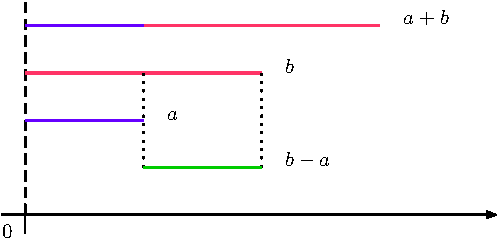
\includegraphics[scale=1]{addsub.pdf}
\end{figure}
$\bullet$ For the sum and difference of two line segments, simply lay them out on the same line, end to end for the sum, or overlapping for the difference.
\end{proof}
\end{frame}


\begin{frame}
\frametitle{The Real Cartesian Plane}
\begin{proof}[Proof of Theorem]\let\qed\relax
\begin{figure}[hbtp]
\centering
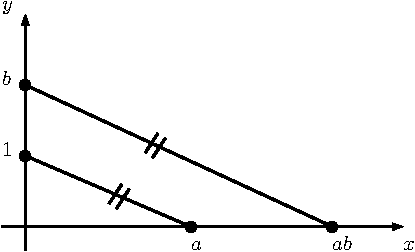
\includegraphics[scale=1]{mult.pdf}
\end{figure}
$\bullet$ For the product, lay the segment $a$ on the $x$-axis, and the segments $1$, $b$ on the $y$-axis. Draw the line from $1$ to $a$, which will have equation $y=-a^{-1}x+1$. The parallel line that passes through $b$ is given by $y=-a^{-1}x+b$ and has $x$-intercept $ab$.
\end{proof}
\end{frame}



\begin{frame}
\frametitle{The Real Cartesian Plane}
\begin{proof}[Proof of Theorem]\let\qed\relax
\begin{figure}[hbtp]
\centering
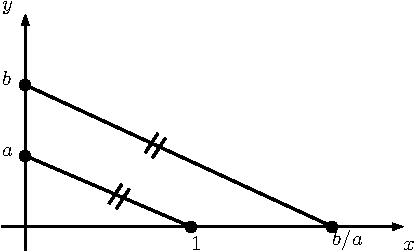
\includegraphics[scale=1]{div.pdf}
\end{figure}
$\bullet$ For the quotient, put $1$ on the $x$-axis, and $a,b$ on the $y$-axis. A similar construction as for the product gives the point $b/a$ on the $x$-axis.
\end{proof}
\end{frame}



\begin{frame}
\frametitle{The Real Cartesian Plane}
\begin{proof}[Proof of Theorem]\let\qed\relax
\begin{figure}[hbtp]
\centering
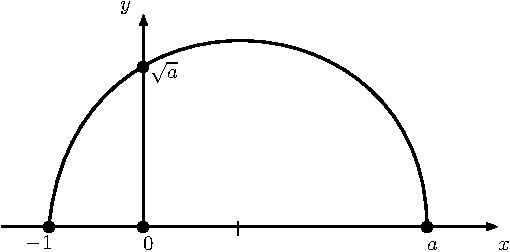
\includegraphics[scale=1]{sqrt.pdf}
\end{figure}
$\bullet$ To construct the square root of a segment $a$, lay out $a$ on the positive $x$-axis, and $-1$ on the negative $x$-axis. Bisect the segment from $-1$ to $a$, and draw the semicircle having that segment as diameter. The circle has equation $\left(x - \frac{a-1}{2}\right)^2 + y^2 = \left( \frac{a+1}{2}\right)^2 $ and $y$-intercept $\sqrt{a}.$
\end{proof}

\end{frame}



\begin{frame}
\frametitle{The Real Cartesian Plane}
\begin{proof}[Proof of Theorem]
To summarize, we have shown how all the field operations $+,-, \cdot , \div$ can be recovered by the mere use of a ruler and a compass where we use lengths that correspond to the coefficients of equations and a unit length of $1$. Moreover we have shown how we can extract the square root of a positive number by using a ruler and a compass. 
\end{proof}
\end{frame}


\begin{frame}
\frametitle{The Real Cartesian Plane}
\begin{prop} In a circle of radius $1$, the length of the side of a regular decagon is $\frac{1}{2}( \sqrt{5}-1).$
\end{prop}

\end{frame}

\begin{frame}
\frametitle{The Real Cartesian Plane}
\begin{proof}[Proof of Proposition] 

\begin{figure}[hbtp]
\centering
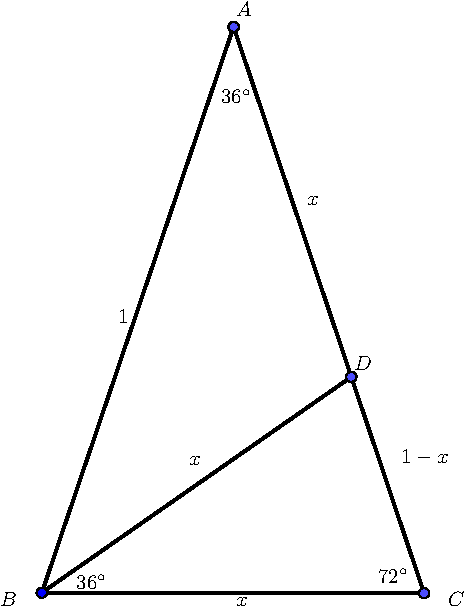
\includegraphics[scale=.4]{construction.pdf}
\end{figure}
$\bullet$ The triangles $ABD$ and $BCD$ are isosceles and $BCD \sim ABC$.
\pause
\newline
$\bullet$ $BD=x$, $AD=x$ and $CD=1-x$. 
\pause
\newline
$\bullet$ Ratio of corresponding sides of similar triangles yields $\frac{1-x}{x}= \frac{x}{1} \implies x^2+x-1=0 \implies x= \frac{1}{2}( \sqrt{5}-1).$

\end{proof}
\end{frame}

\begin{frame}
\frametitle{The Real Cartesian Plane}
\begin{rem} With a little bit of more work, this result allows us to give an analytic proof of the construction of the regular pentagon (seen in a previous talk). 
\end{rem}
\end{frame}


\begin{frame}
\frametitle{The Real Cartesian Plane}
Idea behind analytic proof for regular pentagon:
\pause
\begin{figure}[hbtp]
\centering
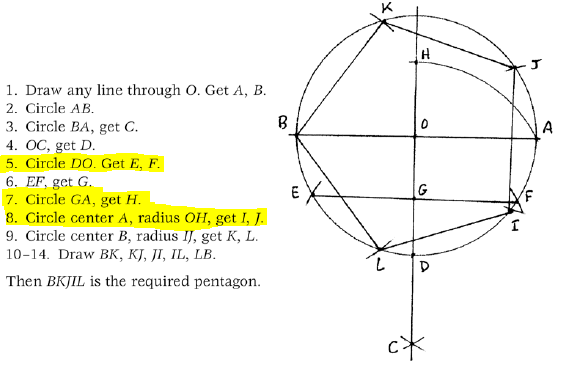
\includegraphics[scale=.5]{idea.png}
\end{figure}
\pause
$\bullet$ $0A=1$, then $0G=1/2$ and (Pythagoras) $GA= \sqrt{5}/2$, hence $0H= \frac{1}{2}( \sqrt{5}-1)$. Thus $A,I,J$ are vertices of regular decagon, so $IJ$ is a side of a regular pentagon.
\end{frame}



\begin{frame}
\frametitle{The Real Cartesian Plane}
\begin{prop}The length of the chord $d$ of a circle of radius $1$ subtending an angle $\alpha$ at the center of the circle is given by \begin{align*}
d= \sqrt{2-  2 \cos \alpha}.
\end{align*}
\begin{figure}[hbtp]
\centering
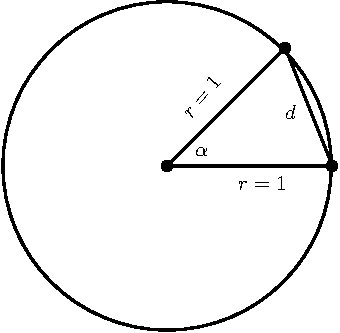
\includegraphics[scale=.8]{lawcosine.pdf}
\end{figure}
\end{prop}
\end{frame}


\begin{frame}
\frametitle{The Real Cartesian Plane}
\begin{prop}The length of the chord $d$ of a circle of radius $1$ subtending an angle $\alpha$ at the center of the circle is given by \begin{align*}
d= \sqrt{2-  2 \cos \alpha}.
\end{align*}
\end{prop}
\pause
\begin{rem} We didn't use this Proposition to compute the side length of the regular decagon because by ruler and compass construction we do not know what $\cos{36^\circ}$ is.
\end{rem}
\pause
\begin{proof}
The law of cosines gives $d^2=1^2+1^2-2 \cos \alpha$.  \\
($c^2= a^2 + b^2-2ab \cos \gamma$.)
\end{proof}
\end{frame}


\begin{frame}
\frametitle{The Real Cartesian Plane}
\begin{prop} In a circle of radius $1$, the side of the regular pentagon is $\frac{1}{2} \sqrt{10-2 \sqrt{5}}$.
\end{prop}
\pause
\begin{proof}
$\bullet$ By the previous Proposition, $d=\sqrt{2-2 \cos 72^\circ}$, since the side of a regular pentagon subtends an angle of $72^\circ$ at the center of the circle.
\pause
\newline
\newline
$\bullet$ Law of cosines applied to the triangle $ABC$ (prop. side length decagon), gives $1^2=1^2+x^2-2x \cos 72^\circ$, where $x= \frac{1}{2}( \sqrt{5}-1)$. 
\pause
\newline
\newline
$\bullet$ Hence $\cos72^\circ = \frac{1}{4}( \sqrt{5}-1)$ and $d= \frac{1}{2}\sqrt{10-2 \sqrt{5}}$.
\end{proof}
\end{frame}


\section{Summary}


\begin{frame}
\begin{center}
\Huge{\color{blue}{\bf{Summary}}}
\end{center}
\end{frame}


\begin{frame}
\frametitle{Summary}
\begin{itemize}
\item We studied the real Cartesian plane.
\pause
\item We revisited some earlier results from the seminar and noticed that this analytic approach is quite potent.
\pause
\item Proofs are rather short and elegant, ideas are clear. 
\pause
\item The relationship between the algebraic and axiomatic approach to geometry is not (yet) clear.
\pause
\item Motivated by the algebraic approach of the real field $\mathbb{R}$, it might be fruitful to study geometries over more general fields. 
\end{itemize}
\end{frame}

\begin{frame}
\begin{center}
\Huge{\color{blue}{\bf{Thank you}}}
\end{center}
\end{frame}



\end{document}
